\documentclass[11pt]{article}
\usepackage{amsmath, amssymb}
\usepackage[margin=1in]{geometry}
\usepackage{booktabs, tabularx, array, xltabular}
\usepackage{enumitem}
\usepackage{xcolor}
\usepackage{pdfpages}
\usepackage[colorlinks=true, linkcolor=blue!60!black, urlcolor=blue!60!black, bookmarksopen=true]{hyperref}
\setlength{\emergencystretch}{3em}
\newcommand{\Ecd}{\mathsf{Ecd}}

\title{\textbf{Protocol v3.1: proofs appendix}\\[4pt]\large Part A: cryptographic and DP guarantees\quad$\cdot$\quad Part B: sensitivity and statistical guarantees\\ Part C: composition across runs and the hockey-stick ledger}
\date{Draft for review}

\begin{document}
\maketitle
\pdfbookmark[1]{Overview}{overview}

\noindent This appendix collects the proofs for protocol v3.1 (honest-but-curious model). Part~A (page~\pageref{partA}) covers the encoding sensitivity, smudging, the worst-case error bound $B_{\mathrm{tot}}$, output privacy (Theorem~1), input and cohort privacy, and correctness. Part~B (page~\pageref{partB}) covers the replace-one sensitivity, operator-norm concentration, the two-stage choice of $(\lambda,\Psi)$, the bound on $\|\boldsymbol\beta\|$, coverage of both intervals, and the bootstrap RSS correction. Part~C (page~\pageref{partC}) proves composition across runs for an adaptive, possibly colluding coalition of researchers (the paper's Proposition \texttt{prop:compose}), with a self-contained R\'enyi filter, and the hockey-stick treatment of the smudging step that the ledger uses (three sums, the reserved share $\xi_L$ of $\varepsilon_L$, and the rule for $\kappa_L$). Its result numbers are those the paper cites as ``proofs, composition appendix''. Sections 4, 7 and 9 of Part~A and S7--S10 of Part~B were added after a second reading of the companion book on the protocol, whose proofs of these results were checked step by step (with the corrections noted where they occur), and include new results (Part~A, Lemma~7.5 and Proposition~7.7; Part~B, Lemma~S0(b), Lemma~S8$'$, Propositions~S10a and S10b, Theorem~S10c). Each part labels every step as exact, first order, asymptotic, numerical or open, and lists its corrections to the specification.

\section*{Status at a glance}

{\small
\begin{xltabular}{\textwidth}{@{}>{\raggedright\arraybackslash}p{3.9cm}>{\raggedright\arraybackslash}p{2.5cm}>{\raggedright\arraybackslash}X@{}}
\toprule
Claim & Status & Notes \\
\midrule
\endfirsthead
\toprule
Claim & Status & Notes \\
\midrule
\endhead
Lemma 1: encoding sensitivity & proven & $\sqrt{2/N}$ and the $\sqrt N$ rounding term are correct \\
Lemma 2: smudging & proven & $\mathrm{SD}\le\|e\|_2/(\sqrt{2\pi}\sigma_1)+4\epsilon/(1-\epsilon)$ with $\sigma_1=\sqrt{\sigma_c^2-2.1^2}$; the per-release form $2^{-\kappa}(1+2^{-80})+2^{-97}$ needs $\sigma_c\ge2^{42}$ (A, Corollary 2.4, corrected from $2^{20}$); the hockey-stick form needs no floor (C, Lemma 5.1) \\
Obligation O1: worst-case $B_{\mathrm{tot}}$ & proven (explicit) & $\approx2^{25.3}$ for the circuit as specified; errors measured in OpenFHE runs stay 6--8 bits below it (no OpenFHE noise estimate is used); assumes (M5) \\
O1 for OpenFHE's gadget, decoupled scales & proven for model (M3$'$) (A, Lemma~4.1) & $\varsigma_\uparrow=2\max_jk_j$, $\varsigma_\downarrow=2k_P$; $B_{\mathrm{tot},2}=2^{26.59}$ at the evaluation setting; match of OpenFHE~1.5.1 with (M3$'$) by code reading; (M5) for OpenFHE's sampler numerical \\
Centre sensitivity, decoupled scales & proven (A, Lemma~4.3) & $\Delta_{x,2}=2^{27.57}$, remainder $\epsilon_x=2^{-36.5}$ covered by the ``$+1$''; exact rounding in $\mathsf{Ecd}$ assumed \\
Decoding offset & proven (A, Proposition~4.5) & $\bar d_2$ between $10^{-8}$ and $5\cdot10^{-6}$; coefficient-domain $d_{\max}\le2^{38.6}$ \\
zCDP of the ideal mechanism; tight conversion & proven & $\rho_{\mathrm{run}}=0.01496$ matches the specification \\
Theorem 1: output privacy & proven (hybrids) & one-sample RLWE for the re-randomizer; plain RLWE for $\mathsf O$'s public-key share, the only key material $\mathsf O$ sends (circular security only if its rotation-key shares were sent); O1; $\mathsf R$'s errors honestly sampled; slack $\gamma$ statistical \\
Composition across runs & proven (C, Theorem 4.2) & any PPT coalition under the filter; runs fixed in advance under rule (N); the ledger charges a run's full cost at admission; RLWE for a finite menu of parameter sets, against non-uniform adversaries; rule (N) with adaptive requests not proved \\
Hockey-stick ledger and $\kappa_L$ & proven (C, Theorem 5.2, Corollary 5.4, Proposition 5.5) & $\kappa_L=22,21,19,17,15$ at $(10,10^{-6},0.1,10^{-3})$ for $\varepsilon_{\mathrm{run}}=0.5,\dots,8$ \\
G1, G2: input and cohort privacy & proven & simulators, up to the cuckoo-hashing failure probability, now bounded (A, Lemma~7.5: $2^{-49.1}$ at $n_R^{\max}=2{,}000$, $\le2^{-40}$ up to load $0.639$; needs an insertion that finds an assignment whenever one exists) and $\mathsf{R}$'s observable aborts \\
G4: disclosure from the Link phase & proven, ROM and CDH (A, Theorem~7.3) & first layer, without circuit privacy; second layer (\textsc{SanitizeBFV}) proven for the textbook BFV model (A, Proposition~7.7: evaluation noise $\le2^{-31}$ after the switch); OpenFHE's BFVrns not checked against the model \\
Soundness of \textsc{Calibrate}; standard simulation with output; $\mathsf{O}$'s work & proven (A, Section~9) & the run computes its DP functionality against $\mathsf{R}$ when the functionality outputs the centred residue modulo $q_0$; $\Omega(n_{\mathrm{Sc}})$ reads in a cell-probe model \\
Correctness (no wraparound) & proven & failure probability $\le\delta_B+2N e^{-50}$ per release; no condition at the earlier levels (A, Proposition~8.1) \\
S1: replace-one sensitivity & proven, exact for $d_O\ge2$ & triu and Frobenius suprema are equal; regime 3 reduces to three cubics; $d_O=1$ is valid but conservative \\
When $\mathbf y^\top\mathbf y$ is free & partly proven & exact criterion; free if $w\le2(r+o)$, never free if $w>3(r+o)$; boundary in between only numerical \\
S2: operator-norm radius & proven (one-sided) & $r_1$ valid for the event Algorithm 6 uses; about $1.55\times$ conservative \\
S7: exact radius & proven & exact level with fresh draws; transfer to the lattice noise with the TV constant now proved (S0) \\
S8: switch-off & bracket proven; size of the bias partly & bracket tight among Gram matrices with a given $\lambda_{\min}$; spectral bound on the bias by Sudakov--Fernique; empirical factors $1.2$/$1.4$ not proved \\
S9: mechanism bias & proven, explicit constants & leading term, ridge, decay in $\lambda$ \\
S10: FWS $\hat s^2$; clipping; full-record $\Delta$ & proven & plug-in RSS biased by $-\sigma^2(\mathrm{tr}\,\mathbf P+\hat\beta^\top M_\chi\hat\beta)$; interval valid under binding clipping with a public variance bound; full-record $\Delta$ exact: closed form for blocks of dimension $\ge2$, enumeration over five faces for a block of dimension $1$; full-record circuit's $B_{\mathrm{tot}}$, $\Delta_x$ and offset re-derived (S10e) \\
S3: two-stage $(\lambda,\Psi)$ & proven & independent of the stage-2 noise; closed form for $\lambda_O$ \\
S4: bound on $\|\boldsymbol\beta\|$ & proven & holds for the projection coefficient with no model assumed \\
S5: coverage & partly first order & Wald remainder bounded exactly; plug-in variance first order; normality of the sampling term asymptotic \\
S6: bootstrap RSS correction & proven to first order & removes the $O(\sigma^2)$ bias up to $O(\sigma^4)$; constants not explicit \\
\bottomrule
\end{xltabular}}

\section*{Corrections to the specification}
Both parts found claims in \texttt{protocol\_v31.tex} that need to change. The most consequential:
\begin{enumerate}[nosep]
  \item \textbf{The CKKS scale is undersized.} Flooding the whole error in $\ell_2$ needs $\log_2\Omega\approx61.5$ for the circuit as specified, not $52.5$. A restructured circuit brings this down to $\approx57.2$; adding encoding at scale $2^{60}$ by $\mathsf R$ brings it to $\approx53.7$. Calibrate must use the data-independent worst-case bound, never OpenFHE's noise estimate.
  \item \textbf{The centre of the mechanism.} The ideal mechanism must be centred at the noiseless circuit output, not at $\Ecd(\mathbf z)$. Its sensitivity rises by a relative $2^{-33}$. $\Omega$ must be the exact final scale of the circuit.
  \item \textbf{$\delta$ accounting.} The per-release statistical distance is $2^{-\kappa}(1+2^{-80})+2^{-97}$, for $\sigma_c\ge\max\{2^\kappa B_{\mathrm{tot}}/\sqrt{2\pi},2^{42}\}$ (the floor $2^{20}$ stated earlier is too small for the factor $1+2^{-80}$). For a single $(\varepsilon,\delta)$ statement, the slack enters with a factor $(1+e^{\varepsilon})$. Across runs, the ledger charges a run's full cost at admission and accounts the smudging step in hockey-stick divergence (Part~C).
  \item \textbf{Assumptions.} RLWE is needed in two forms. Disclosure G4 needs circuit privacy of $\mathsf O$'s BFV replies; the modulus switch alone is heuristic. G1 and G2 need explicit assumptions and the hashing slack.
  \item \textbf{Algorithm 6.}
    \begin{itemize}[nosep]
      \item The radius comment should be one-sided, or use $\ln(2/\alpha_L)$.
      \item $U_{yy}$ spends $\alpha_U$ twice, and $\sigma_{yy}$ is undefined.
      \item $\boldsymbol\beta$ must be defined as a working-model or projection coefficient on the clipped data, and the homoskedastic variance fails when clipping binds.
      \item The bootstrap needs truncation, since the moments do not exist otherwise.
      \item The bias bound $\bar b_j$ is first order only.
      \item The private $\|\boldsymbol\beta\|$ bound is usually infinite while the ridge is active.
      \item The specification should state whether coverage is conditional on the gate.
    \end{itemize}
  \item \textbf{Smaller points.}
    \begin{itemize}[nosep]
      \item The sampler needs a rational $\sigma_c^2$ and a defined notion of constant time.
      \item The modulus switch to $q_0$ is a no-op after two rescales.
      \item The printed $\Delta=86.18$ comes from unrounded bounds.
      \item The earlier paper's ``$\mathbf y^\top\mathbf y$ is free'' and ``Frobenius is conservative'' are false in general.
    \end{itemize}
\end{enumerate}

\section*{Open items}
\begin{itemize}[nosep]
  \item Full proofs for the two improved circuit variants; a concrete constant-time exact sampler. (Adaptive composition across runs is proved in Part~C; rule (N) with adaptively chosen requests is not. No wraparound needs no condition at the earlier levels; the chain is sized by \textsc{Calibrate}, which is proved sound.) Whether OpenFHE's BFVrns satisfies the BFV model of the $B_\psi$ bound. (The cuckoo insertion now falls back to augmenting paths, so Lemma~7.5 of Part~A covers it.)
  \item The free-set boundary for $\mathbf y^\top\mathbf y$; a closed form for $\Delta$ with $\mathbf y^\top\mathbf y$ when $d_O=1$; explicit constants for S6; a guarantee for the data-driven variance when clipping binds (a public bound gives a valid interval, S10); a spectrum-sharp bound on the downward bias of $\lambda_{\min}$ (S8).
  \item Sixteen citation details are flagged in the two parts for verification, among them theorem numbers in Canonne et al.\ (2020), Vershynin, and Boucheron, Lugosi and Massart.
\end{itemize}

\clearpage
\phantomsection\label{partA}
\pdfbookmark[1]{Part A: cryptographic and DP guarantees}{partA}
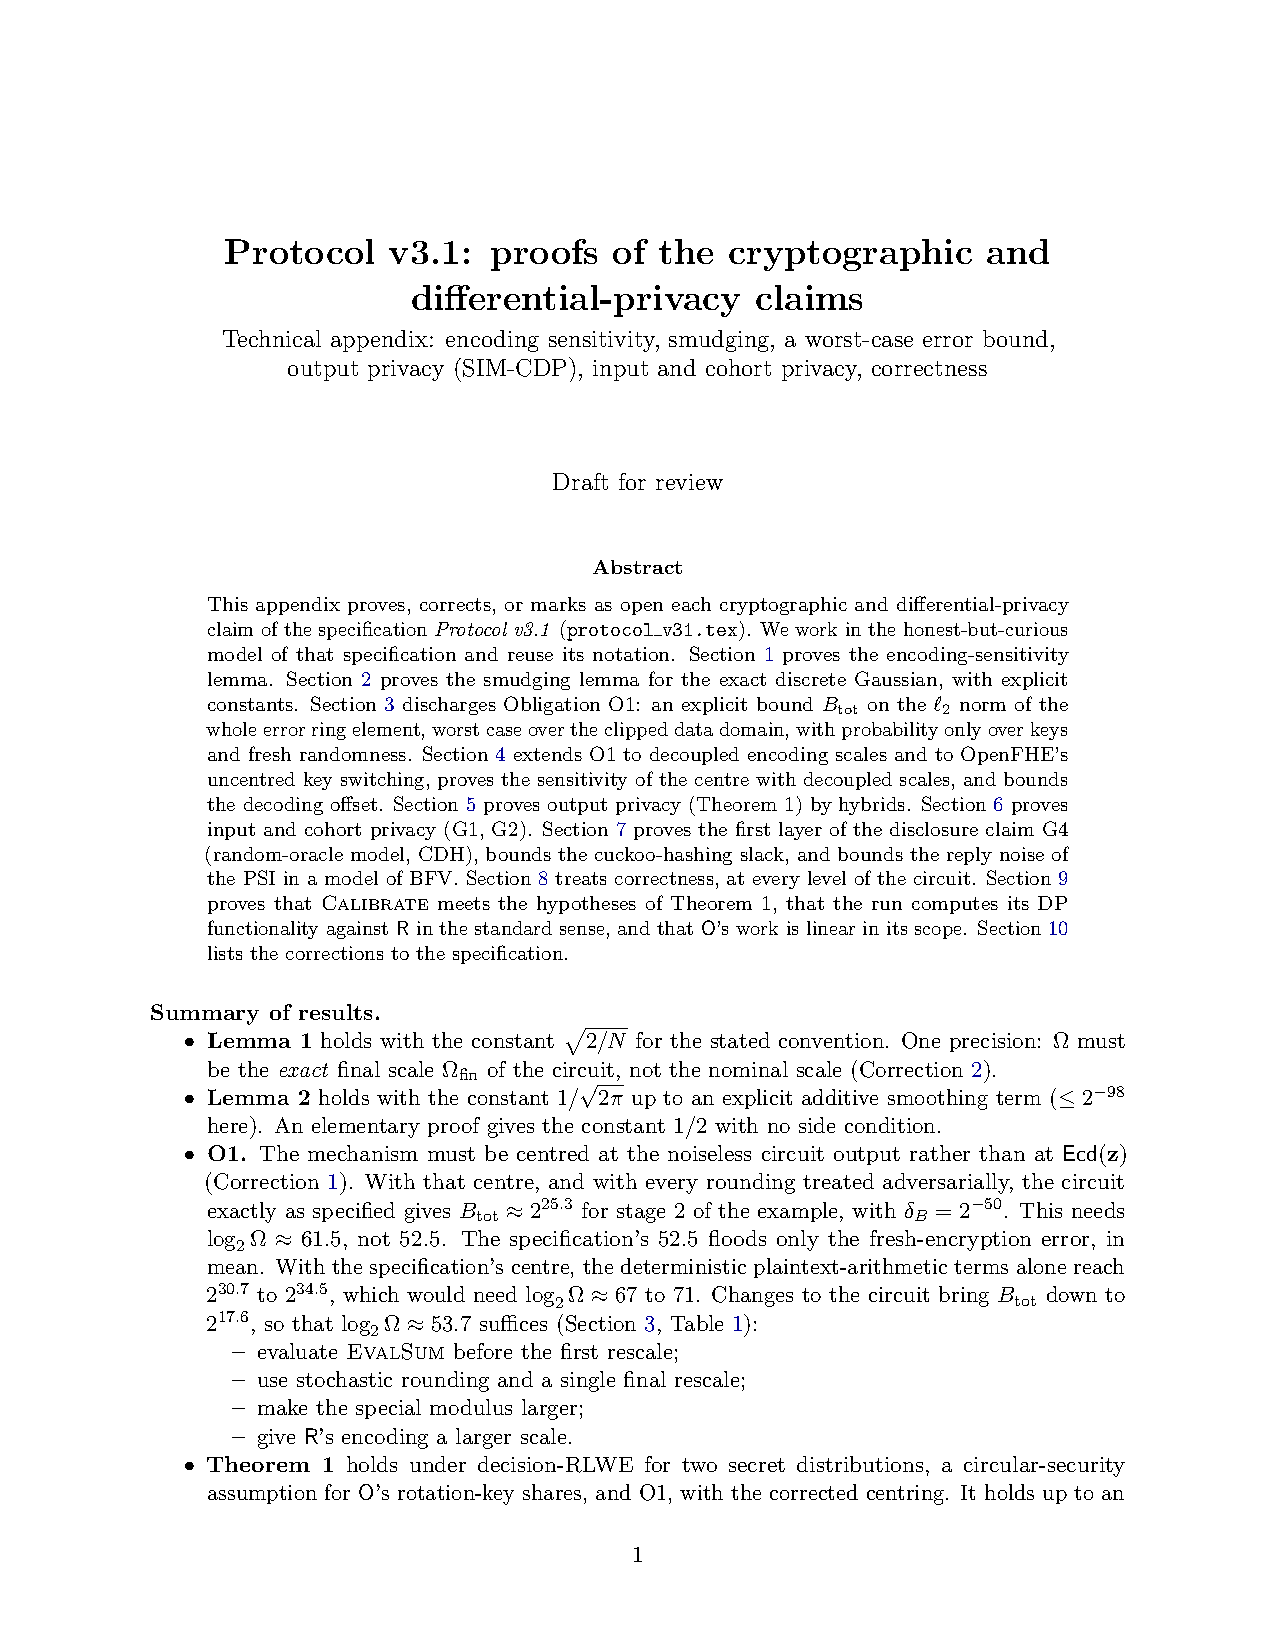
\includepdf[pages=-]{crypto_proofs.pdf}
\phantomsection\label{partB}
\pdfbookmark[1]{Part B: sensitivity and statistical guarantees}{partB}
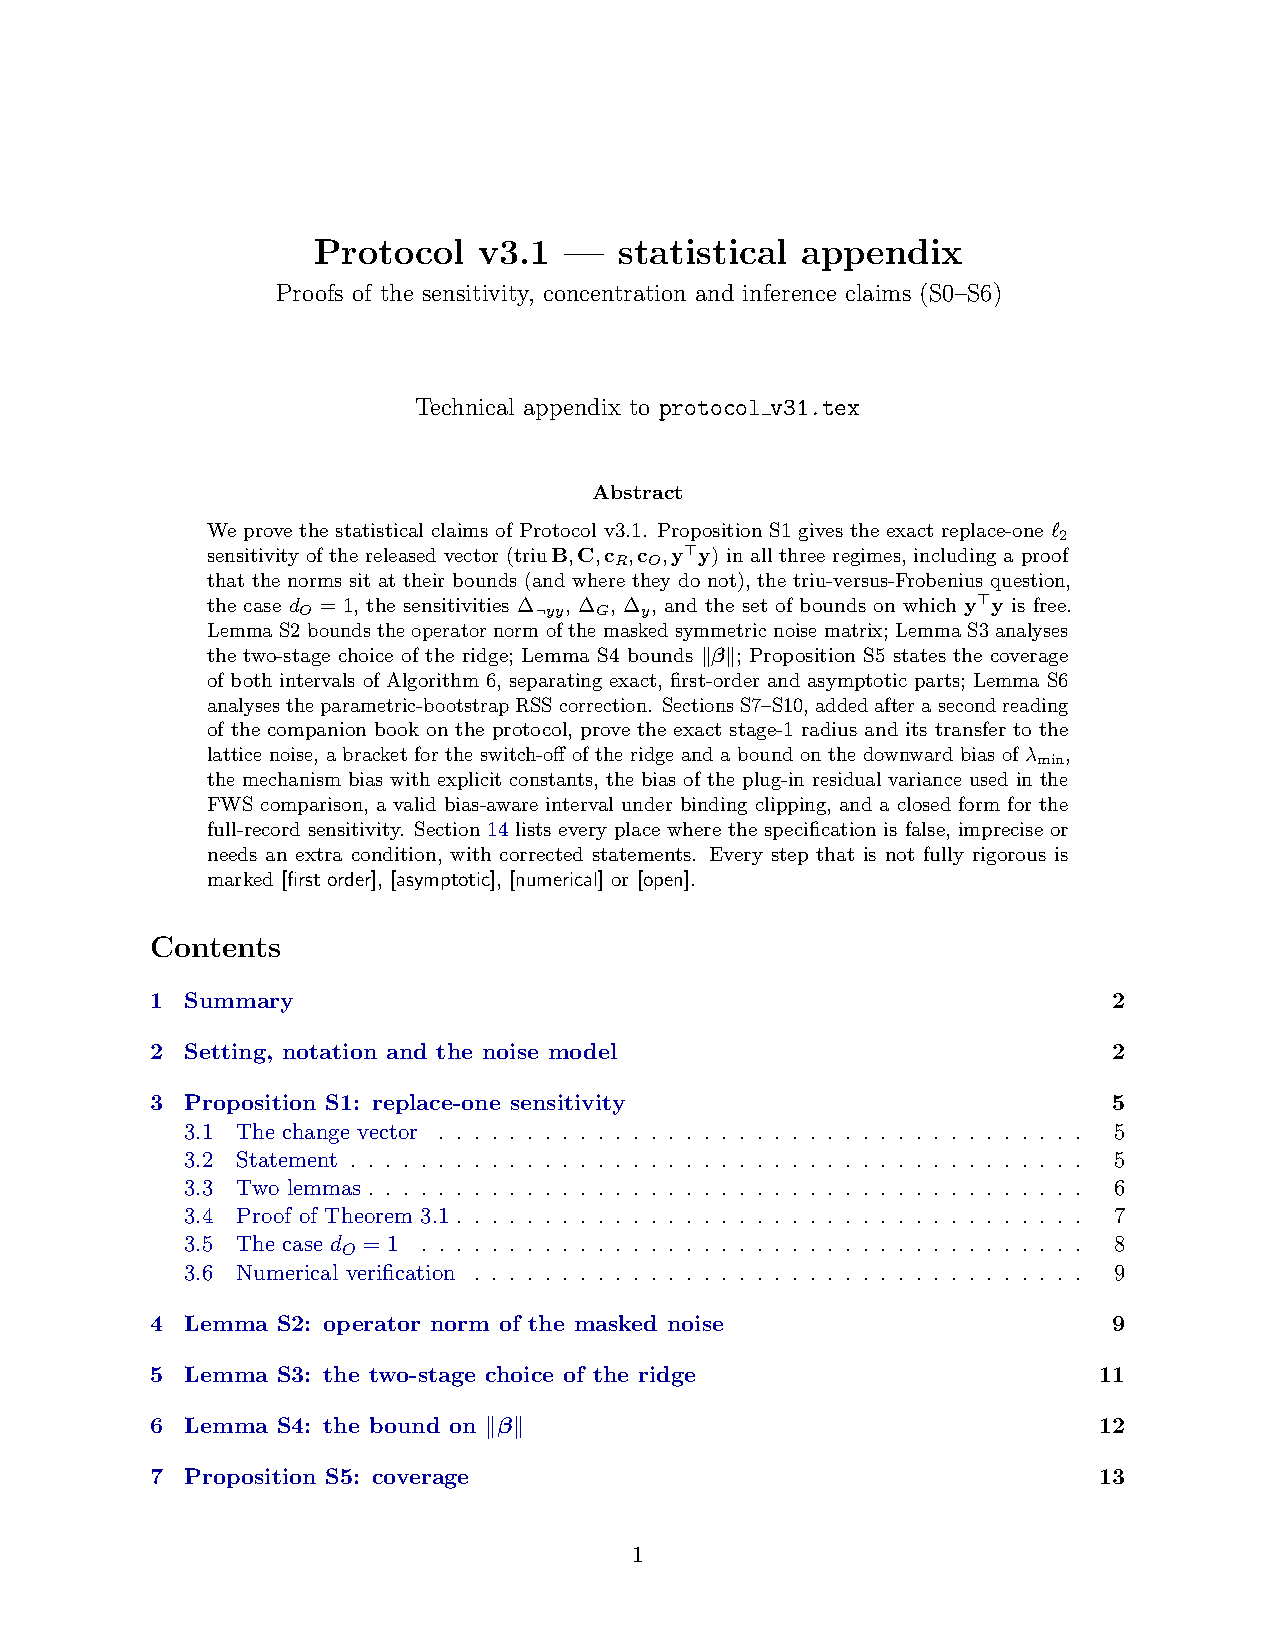
\includepdf[pages=-]{stats_proofs.pdf}
\phantomsection\label{partC}
\pdfbookmark[1]{Part C: composition across runs and the hockey-stick ledger}{partC}
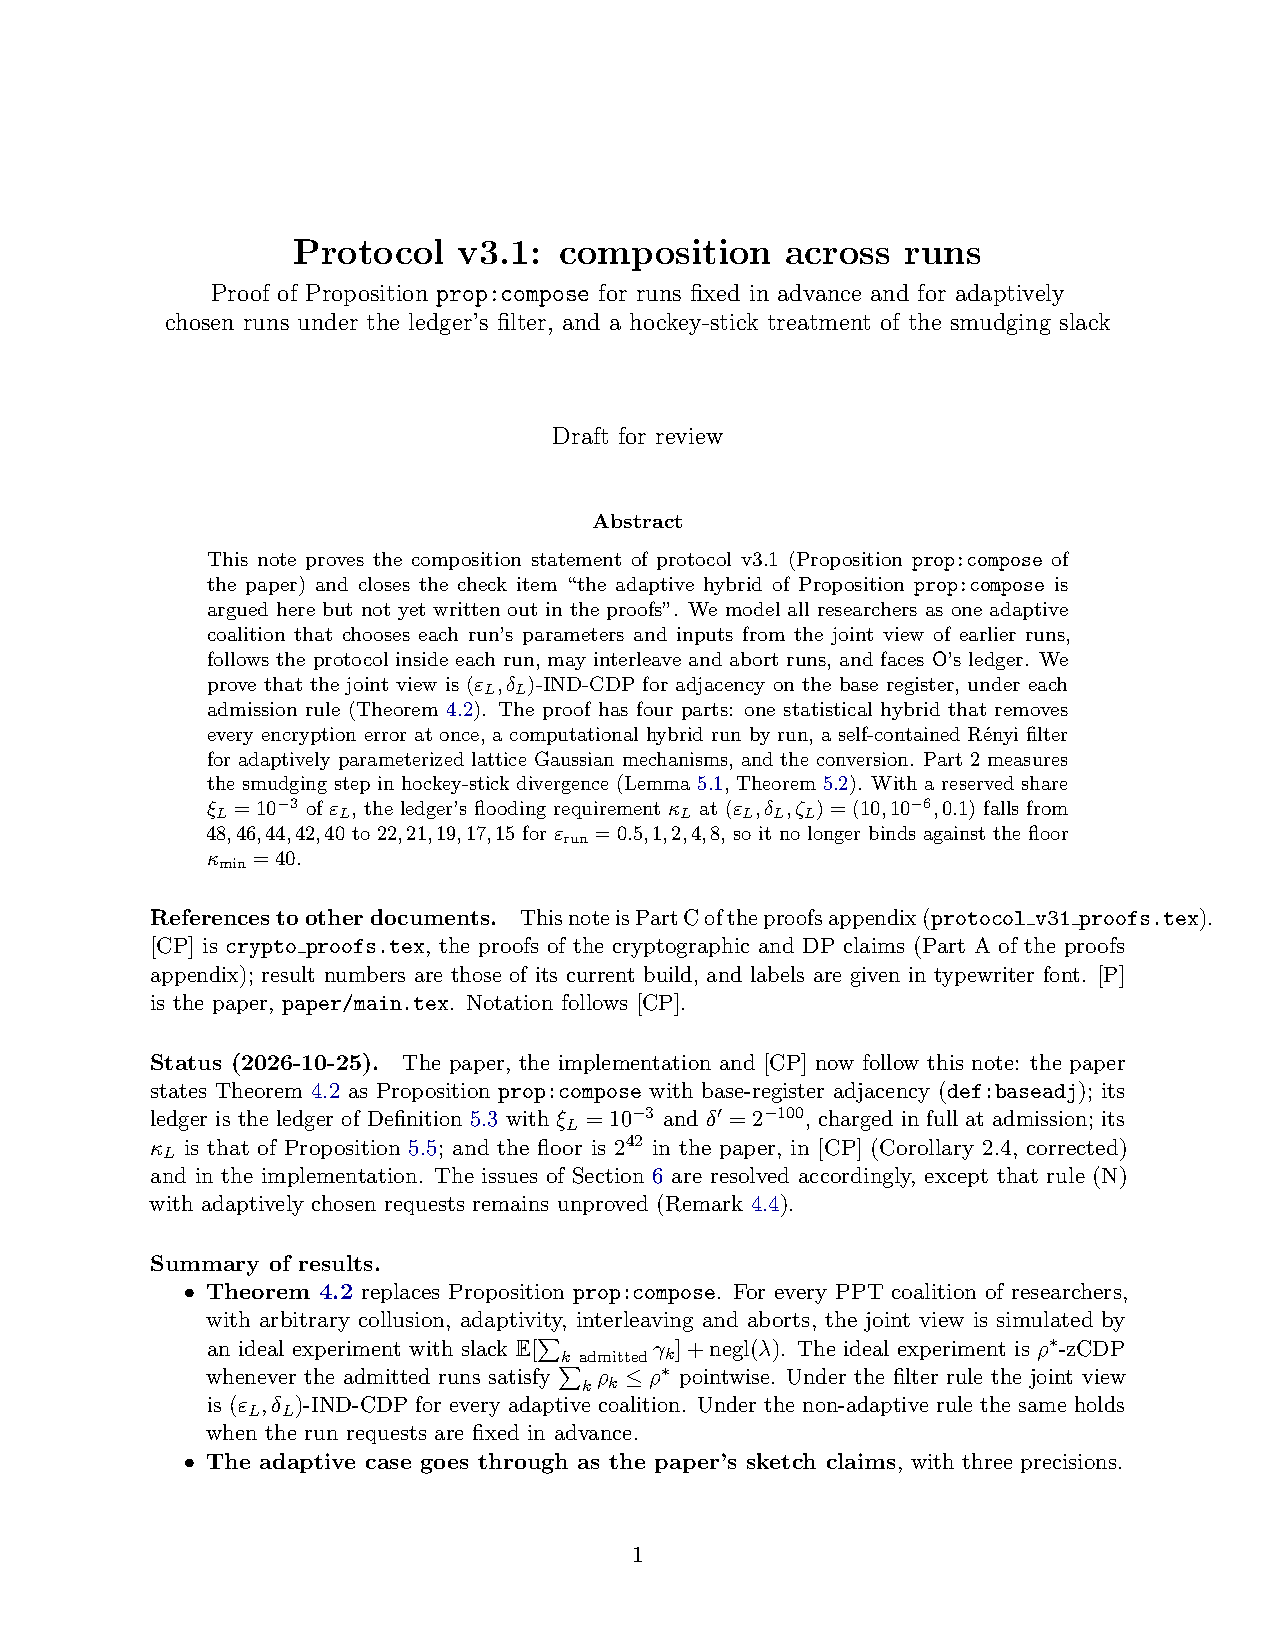
\includepdf[pages=-]{composition/composition_proof.pdf}
\end{document}
